\documentclass[10pt]{amsart}
%\include{amsmath}
\usepackage{mathtools}
\usepackage{amsmath}  
\usepackage{amssymb}  % gives you \mathbb{} font
\usepackage{dsfont}	% gives you \mathds{} font

%                   Math Blackboard Bold Symbols

\newcommand\Cb{\mathds{C}}
\newcommand\Eb{\mathds{E}}
\newcommand\Fb{\mathds{F}}
\newcommand\Gb{\mathds{G}}
\newcommand\Ib{\mathds{I}}
\newcommand\Pb{\mathds{P}}
\newcommand\Qb{\mathds{Q}}
\newcommand\Rb{\mathds{R}}
%\newcommand\Zb{\mathds{Z}}
\newcommand\Nb{\mathds{N}}
\newcommand\Vb{\mathds{V}}
\newcommand\Ub{\mathds{U}}

\usepackage[shortlabels]{enumitem}
\usepackage{amssymb}
\usepackage{bbm}
\usepackage{cancel}
\usepackage{graphicx,subfig}

\graphicspath{ {./images/} }

\newcommand{\D}{\mathrm{d}}
\DeclareMathOperator{\E}{e}
\DeclareMathOperator{\I}{i}


\begin{document}

\noindent
\text{Hunter Lybbert} \\
\text{Student ID: 2426454} \\
\text{11-22-24} \\
\text{AMATH 561}
\title{Problem Set 7}
\maketitle

{\it Note: Exercises 1-4 are from Matt Lorig's
notes (link on course website).}
\\

\noindent {\bf 1.} Exercise 4.1. \\
A six-sided die is rolled repeatedly. Which of the following are Markov chains? For those
that are, find the one-step transition matrix.\\

\begin{enumerate}[(a)]
\item $X_n$ is the largest number rolled up to the $n$th roll. \\

\noindent
\textit{Solution:} \\
It helps me to visualize this graphically. 
Let each state be a node with directed edges going from a given state to all reachable states from the current state.
\begin{figure}[h]
	\centering
	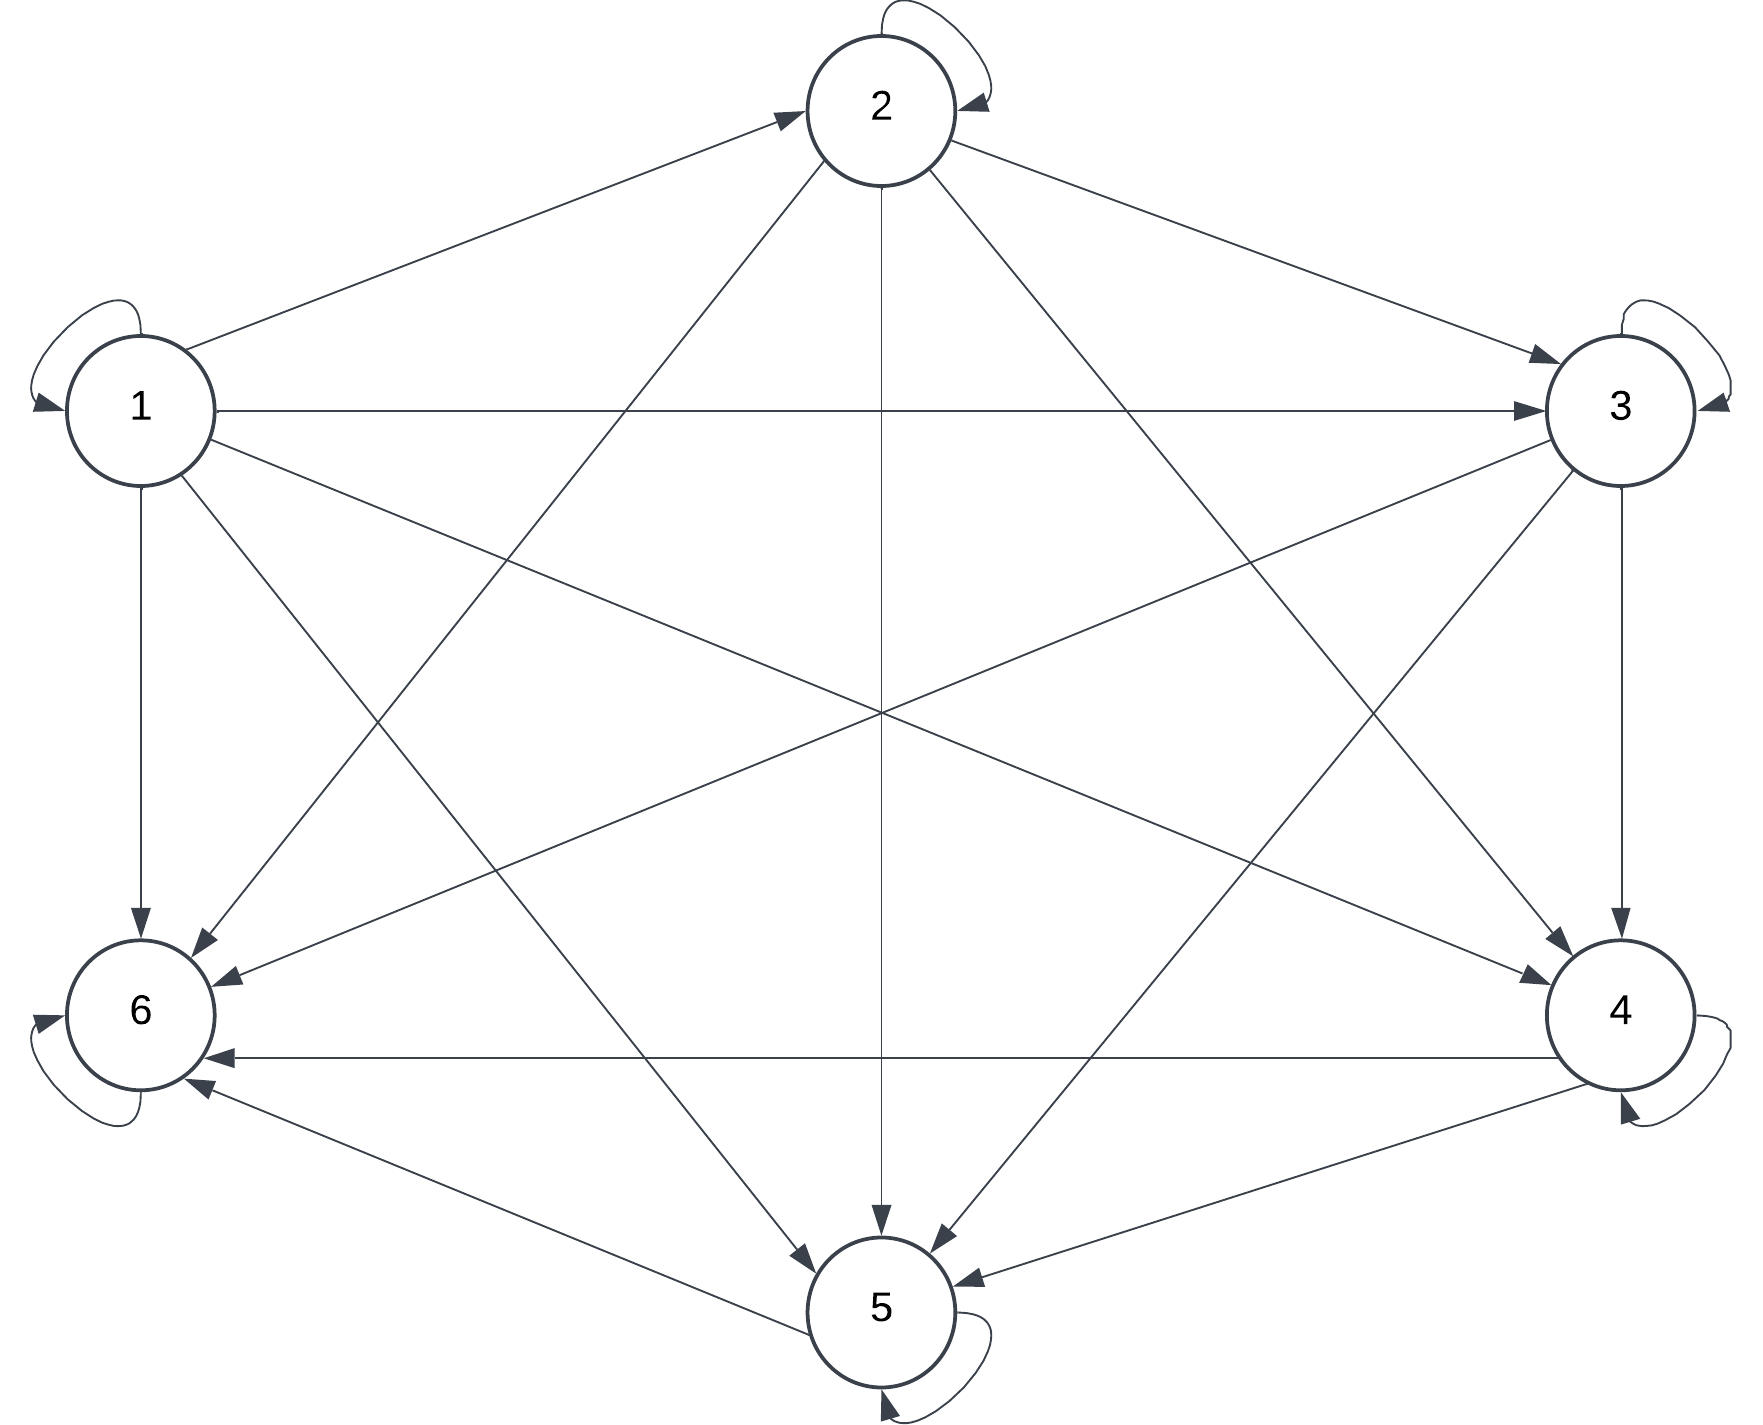
\includegraphics[scale=0.5]{one_part_a_markov_graph.png}
	\caption{
		A graphical representation of the Markov Chain in problem 1 part (a).
	}\label{fig:f1}
\end{figure}
If each directed edge in Figure \ref{fig:f1} is equally likely, then we can construct the following transition matrix
\begin{align*}
P = 
\begin{bmatrix}
1 /6 & 1 /6 & 1 /6 & 1 /6 & 1/6 & 1/6 \\
0 & 1/5 & 1/5 & 1/5 & 1/5 & 1 /5 \\
0 & 0 & 1/4 & 1/4 & 1/4 & 1/4 \\
0 & 0 & 0 & 1/3 & 1/3 & 1/3 \\
0 & 0 & 0 & 0 & 1/2 & 1/2 \\
0 & 0 & 0 & 0 & 0 & 1 \\
\end{bmatrix}.
\end{align*}
From the transition matrix it is easy to see this is a Markov chain.
This is due to the fact that the rows sum to $1$ and the probability of moving to a new state only depends on our current state. \\
\qed \\


\item $X_n$ is the number of sixes rolled in the first $n$ rolls. \\

\noindent
\textit{Solution:} \\
The transition matrix for this scenario can be written as
\begin{align*}
P =
\begin{bmatrix}
5/6 & 1/6 & 0 & 0 & \dots \\
0 & 5/6 & 1/6 & 0 & \dots \\
0 & 0 & 5/6 & 1/6 & \ddots\\
\vdots & \vdots & \ddots & \ddots & \ddots\\
\end{bmatrix}.
\end{align*}
Since we can write $X_n = X_{n - 1} + \xi_n$ where $\xi_n$ is 1 if the $n$th role is a 6 or 0 otherwise.
Therefore $\xi_n$ is Bernoulli distributed with probability of success $p = 1/6$.
Let the current state be denoted as $\ell$.
The state space is $\mathbb N \cup \{0\}$.
Furthermore we can say if $X_n = \ell$ we denote the following
$$
P(X_{n + 1} = \ell + 1 | X_n = \ell) = 1 / 6
$$
if the next role is a 6 and
$$
P(X_{n + 1} = \ell | X_n = \ell) = 5 / 6
$$
if the next role is not a 6.
Graphically that can be represented as seen in Figure \ref{fig:f2}
\begin{figure}[h]
	\centering
	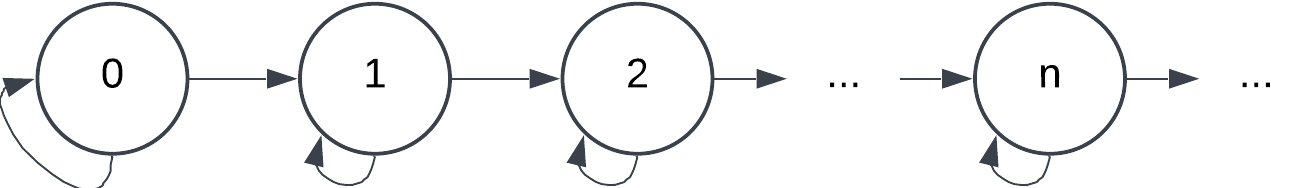
\includegraphics[scale=0.5]{one_part_b_markov_graph.png}
	\caption{
		A graphical representation of the Markov Chain in problem 1 part (b).
	}\label{fig:f2}
\end{figure}
Where the self returning edge has probability $5/6$ and the edge advancing from one state to the next higher state has probability $1/6$.
Now we can conclude this is a Markov chain because the probability of moving to a particular state is only determined by the current state we are in.
Additionally the rows of our matrix sum to 1 which satisfies our other criteria. \\
\qed \\


\item At time $n$, $X_n$ is the time since the last six was rolled. \\

\noindent
\textit{Solution:} \\
Each step is $5/6$ chance of not rolling a 6 therefore increasing $X_n$ and a $1/6$ chance of rolling a 6 therefore returning to the beginning state.
If I may say so myself, this is depicted clearly in the directed graph in Figure \ref{fig:f3}. \\
\begin{figure}[h]
	\centering
	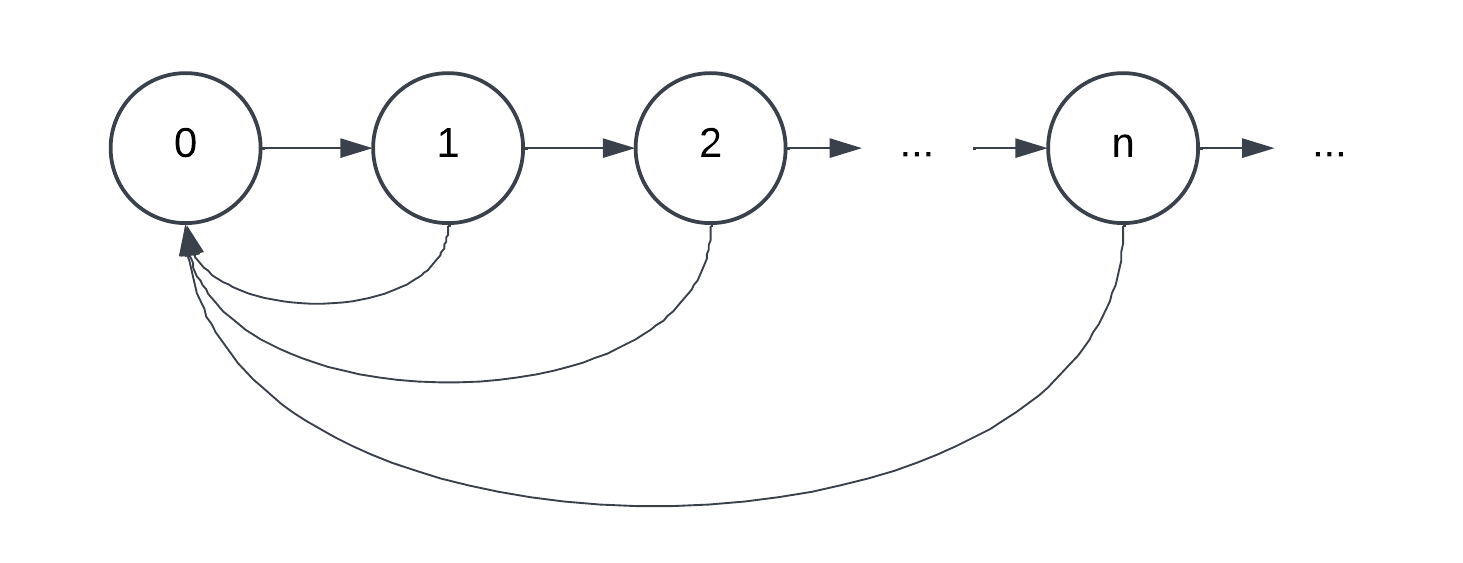
\includegraphics[scale=0.5]{one_part_c_markov_graph.png}
	\caption{
		A graphical representation of the Markov Chain in problem 1 part (c).
	}\label{fig:f3}
\end{figure} \\

\noindent
The one step transition matrix can be written as
\begin{align*}
P =
\begin{bmatrix}
1/6 & 5/6 & 0 & 0 & \dots \\
1/6 & 0 & 5/6 & 0 & \dots \\
1/6 & 0 & 0 & 5/6 & \ddots\\
\vdots & \vdots & \ddots & \ddots & \ddots\\
\end{bmatrix}.
\end{align*}
Once again, observe we have rows that sum to 1 and the probability of moving from one state to another only depends on which state we are currently in. \\
\qed \\


\item At time $n$, $X_n$ is the time until the next six is rolled. \\

\noindent
\textit{Solution:} \\
Suppose $X_1 = k$ meaning we are going to role a 6 in $k$ roles.
Then we know that $X_2 = k - 1, ..., X_k = 1$.
Thus the $k + 1$ role is a 6 and we no longer have definitive information about time until the next 6 will be rolled.
Let's consider $X_{k + 1} = \ell$, $\ell \in \mathbb N$. Then there are going to be $\ell - 1$ non 6 roles followed by a single role of 6.
The probability of $\ell - 1$ non 6 roles is $\big(\frac 5 6 \big)^{\ell - 1}$ then we would multiply by an additional $1/6$.
We can represent this uncertainty for the state of $X_{k+1}$ as 
$$P(X_{k + 1} = \ell) = \bigg(\frac 5 6 \bigg)^{\ell - 1}\frac 1 6.$$
Notice, this is just a geometric distribution.
Therefore, the one step transition matrix can be written as
\begin{align*}
P =
\begin{bmatrix}
1/6 & (5/6)1/6 & (5/6)^2 1/6 & (5/6)^3 1/6 & \dots \\
1 & 0 & 0 & 0 & \dots \\
0 & 1 & 0 & 0 & \ddots\\
0 & 0 & 1 & 0 & \ddots\\
\vdots & \vdots & \ddots & \ddots & \ddots\\
\end{bmatrix}.
\end{align*}
Since the first row of the matrix is just a geometric distribution it sums to 1 and the others sum to 1 trivially.
Additionally, the probability of moving from one state to another is fully determined by the current state, this is indeed a Markov Chain.
\qed \\

\end{enumerate}
\newpage


\noindent {\bf 2.} Exercise 4.2. \\
Let $Y_n = X_{2n}$. Compute the transition matrix for $Y$ when

\begin{enumerate}[(a)]
\item $X$ is a simple random walk (i.e., $X$ increases by one with probability $p$ and decreases by $1$ with probability $q$. \\

\noindent
\textit{Solution:} \\
Let's define the one step transition matrix for the random variable $X$ which is a random walk increasing by 1 or decreasing by 1 with probability $p$ and $q$ respectively.
The matrix is
\begin{align*}
\begin{bmatrix}
0 & p & 0 & 0 & 0 & \dots \\
q & 0 & p & 0 & 0 & \dots \\
0 & q & 0 & p & 0 & \dots \\
0 & 0 & q & 0 & p & \dots \\
0 & 0 & 0 & q & 0 & \ddots \\
\vdots & \vdots & \vdots & \ddots & \ddots & \ddots \\
\end{bmatrix}
\end{align*}
Looking at the graph in Figure \ref{fig:f4}
\begin{figure}[h]
	\centering
	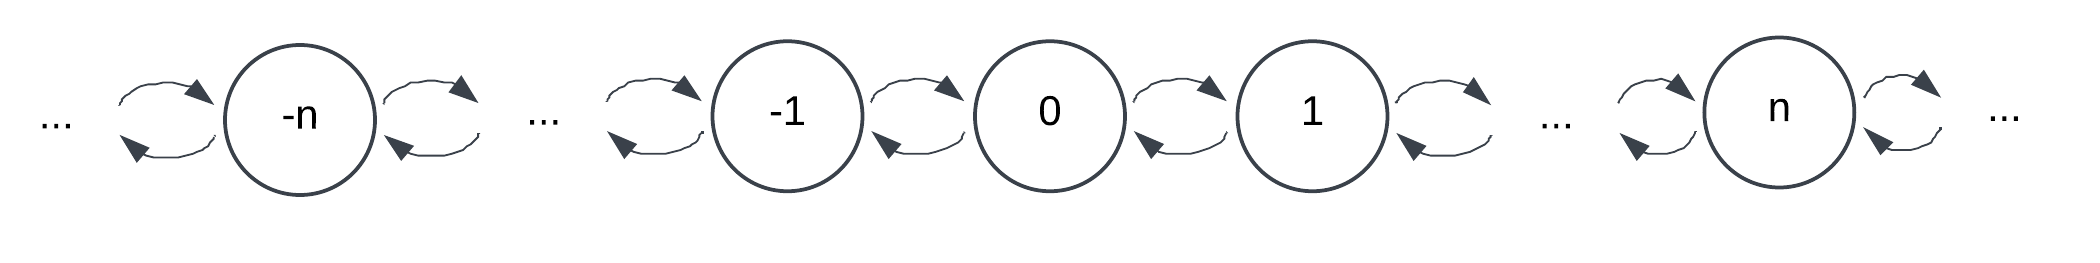
\includegraphics[scale=0.5]{two_part_a_markov_graph.png}
	\caption{
		A graphical representation of the Markov Chain in problem 2 part (a).
	}\label{fig:f4}
\end{figure}
Let $P$ be transition matrix for $X_n$, then transition matrix for $Y_n$ should be $P^2$, also could use kolmogorov equation or something...
\textbf{TODO:} \\
\begin{align*}
\end{align*}


\item $X$ is a branching process where $G$ is the generating function of the number of offspring from each individual. \\

\noindent
\textit{Solution:} \\
\textbf{TODO: Office Hour notes} \\
\begin{enumerate}[--]
\item $G_{i + 1}$ conditioning?
\item $\xi_i$
\item $\sum_i \xi_i \implies E(s^{\sum_i \xi_i})$
\item ends up being $G^i$ maybe
\item (random) $G^i(s) = E( s^{X_{2n+ 1}}| X_{2n} = i)$
\end{enumerate}
\begin{align*}
\end{align*}

\end{enumerate}

\newpage


\noindent {\bf 3.} Exercise 4.3. \\
Let $X$ be a Markov chain with state space $S$ and absorbing state $k$ (i.e., $p(k, j) = 0$ for all $j \in S$).
Suppose $j \rightarrow k$ for all $j \in S$.
Show that all states other than $k$ are transient. \\

\noindent
\textit{Solution:} \\
\textbf{TODO:} \\
This is supposedly a clean quick proof... \\
argue with words...? No needs to be written in mathematical probability terms ... \\
chapman? no \\
Consider a proof by contradiction... actually maybe not though
\begin{align*}
\end{align*}

\newpage


\noindent {\bf 4.}  Exercise 4.4. \\
Suppose two distinct states $i, j$ satisfy
$$
P(\tau_j < \tau_i | X_0 = i) = P(\tau_i < \tau_j | X_0 = j)
$$
where $\tau := {\rm inf}\{n \geq 1: X_n = j\}$.
Show that, if $X_0 = i$, the expected number of visits to $j$ prior to re-visiting $i$ is one. \\

\noindent
\textit{Solution:} \\
\textbf{TODO:} \\
Layer cake representation 
$$
E(X) = \int_0^\infty P(X > t) \D t
$$
but this is a summation in our scenario
\begin{align*}
\end{align*}

\newpage


\noindent {\bf 5. Stationary distribution of Ehrenfest chain.} (a) Let $X_n$ be the number of balls in the left urn at time $n$ (total number of balls in both urns is $r$). At each time step, one of the $r$ balls is picked at random and moved to the other urn. \\

\noindent
(a) Let $G_n(s)$ be the generating function of $X_n$. Derive a formula for $G_{n+1}$ as a function of $G_n$. \\

\noindent
\textit{Solution:} \\
\textbf{TODO:} \\
\begin{align*}
\end{align*}

\noindent
(b) Let $G(s)= \lim_{n \to \infty}  G_n(s)$. Use the relation in part a) to derive an equation for $G$. Solve it and find $G$. \\

\noindent
\textit{Solution:} \\
\textbf{TODO:} \\
\begin{align*}
\end{align*}

\noindent
(c) Find the stationary distribution $\pi$ of Ehrenfest chain. What is the connection between $G$ and $\pi$? \\

\noindent
\textit{Solution:} \\
Stationary distr? \\
\textbf{TODO:} \\
\begin{align*}
\end{align*}

\newpage




\end{document}  
